%% CS5480 Deep Learning — Kaggle Competition Presentation
\documentclass[aspectratio=169]{beamer}

\usetheme{Copenhagen}
\usecolortheme{default}

\usepackage{graphicx}
\usepackage{booktabs}
\usepackage{amsmath}
\usepackage{amssymb}
\usepackage{xcolor}

\setbeamertemplate{navigation symbols}{}
\setbeamertemplate{caption}[numbered]
\setbeamerfont{block title}{size=\small}
\setbeamerfont{block body}{size=\footnotesize}

%% colour accents
\definecolor{iithblue}{RGB}{0,70,140}
\definecolor{iithgold}{RGB}{200,150,0}
\setbeamercolor{structure}{fg=iithblue}
\setbeamercolor{frametitle}{bg=iithblue, fg=white}
\setbeamercolor{block title}{bg=iithblue!85, fg=white}
\setbeamercolor{block body}{bg=iithblue!8}
\setbeamercolor{alerted text}{fg=iithgold}

\author[Neeli \& Meerjumla]{%
  Lochan Surya Teja Neeli (CS25MTECH11015) \and
  Harshavardhan Meerjumla (CS25MTECH11011)}
\title[Binary Classification — CS5480]{%
  Binary Image Classification\\
  with CBAM-Enhanced ResNet, GeM Pooling\\
  and Edge-Map Preprocessing}
\institute[IIT Hyderabad]{Department of CSE, IIT Hyderabad}
\date{CS5480 Deep Learning Hackathon 2026}

\begin{document}

% ── Title ─────────────────────────────────────────────────────────────
\begin{frame}
  \titlepage
\end{frame}

% ═══════════════════════════════════════════════════════════════════════
\section{Problem \& Dataset}
% ═══════════════════════════════════════════════════════════════════════

\begin{frame}[t,shrink=8]{Problem Statement}
  \begin{columns}[T]
    \begin{column}{0.52\textwidth}
      \begin{block}{Competition}
        \footnotesize \textbf{IITH DL Hackathon 2026 (CS5480)}\\
        Binary image classification — \alert{no pretrained weights}\\
        18,000 training images, trained entirely from scratch
      \end{block}
      \smallskip
      \begin{block}{Classification Rule}
        \footnotesize
        \begin{itemize}
          \item \textbf{Class 1}: scene has $\geq1$ sphere \textbf{AND} $\geq1$ cube
          \item \textbf{Class 0}: all other configurations
        \end{itemize}
        The signal is \alert{purely shape} — colour \& background are identical across classes
      \end{block}
    \end{column}
    \begin{column}{0.45\textwidth}
      \begin{block}{Two key challenges}
        \footnotesize
        \begin{enumerate}
          \item \textbf{Destructive augmentation}\\
                \texttt{RandomResizedCrop} can exclude the only sphere or cube $\to$ silent label corruption
          \item \textbf{Colour bias}\\
                Same colours appear in both classes; RGB wastes capacity on spurious cues
        \end{enumerate}
      \end{block}
    \end{column}
  \end{columns}
\end{frame}

\begin{frame}[t,shrink=5]{Dataset}
  \begin{columns}[T]
    \begin{column}{0.44\textwidth}
      \begin{block}{Structure}
        \footnotesize
        \begin{itemize}
          \item \textbf{18,000} labelled training images (9k Class-0 + 9k Class-1, balanced)
          \item \textbf{5,010} unlabelled test images
          \item CLEVR-style 3-D renders: 4 geometric objects on a plain grey background
        \end{itemize}
      \end{block}
      \smallskip
      \begin{block}{Train / Val split}
        \footnotesize 85\% / 15\% random permutation\\
        \texttt{torch.randperm}, \texttt{split\_seed=42}
      \end{block}
    \end{column}
    \begin{column}{0.54\textwidth}
      \centering
      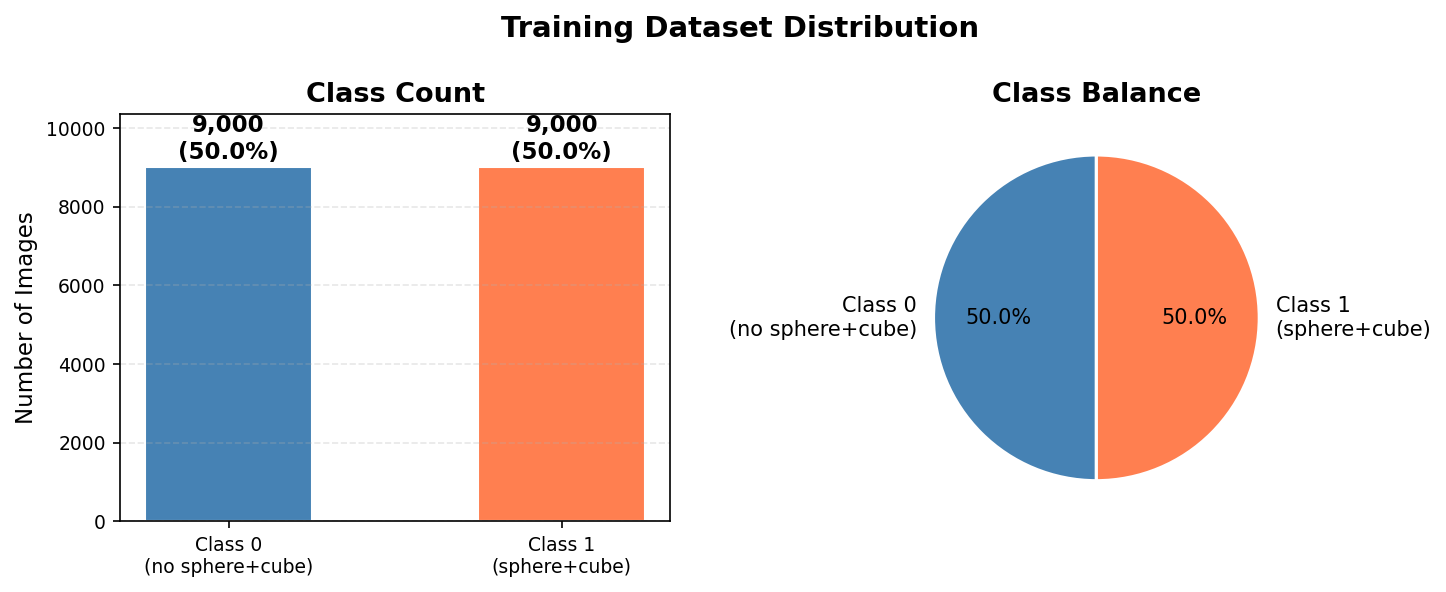
\includegraphics[width=\textwidth,height=0.60\textheight,keepaspectratio]{figures/dataset_distribution.png}
    \end{column}
  \end{columns}
\end{frame}

% ═══════════════════════════════════════════════════════════════════════
\section{ShapePreprocess}
% ═══════════════════════════════════════════════════════════════════════

\begin{frame}[t,shrink=12]{ShapePreprocess: Edge-Map Preprocessing}
  \begin{columns}[T]
    \begin{column}{0.44\textwidth}
      \begin{block}{Pipeline (deterministic, every image)}
        \footnotesize $\text{RGB} \to \text{Grayscale} \to {\times3\,\text{Contrast}}
          \to \texttt{FIND\_EDGES} \to \text{RGB}$
      \end{block}
      \smallskip
      \begin{block}{Why it works}
        \footnotesize
        \begin{itemize}
          \item \textbf{Sphere} $\to$ smooth circular contour
          \item \textbf{Cube} $\to$ sharp rectangular corners
          \item \textbf{Cylinder} $\to$ rounded top, flat sides
        \end{itemize}
        Eliminates colour \& shading entirely.\\
        Normalisation: $\mu\!=\!\sigma\!=\![0.5,0.5,0.5]$
      \end{block}
      \smallskip
      \begin{block}{Augmentations (train only)}
        \footnotesize \texttt{Resize(224)}, \texttt{RandomHorizontalFlip}\\
        \alert{Disabled}: ColorJitter, GaussianBlur, MixUp, CutMix, RandomResizedCrop
      \end{block}
    \end{column}
    \begin{column}{0.54\textwidth}
      \centering
      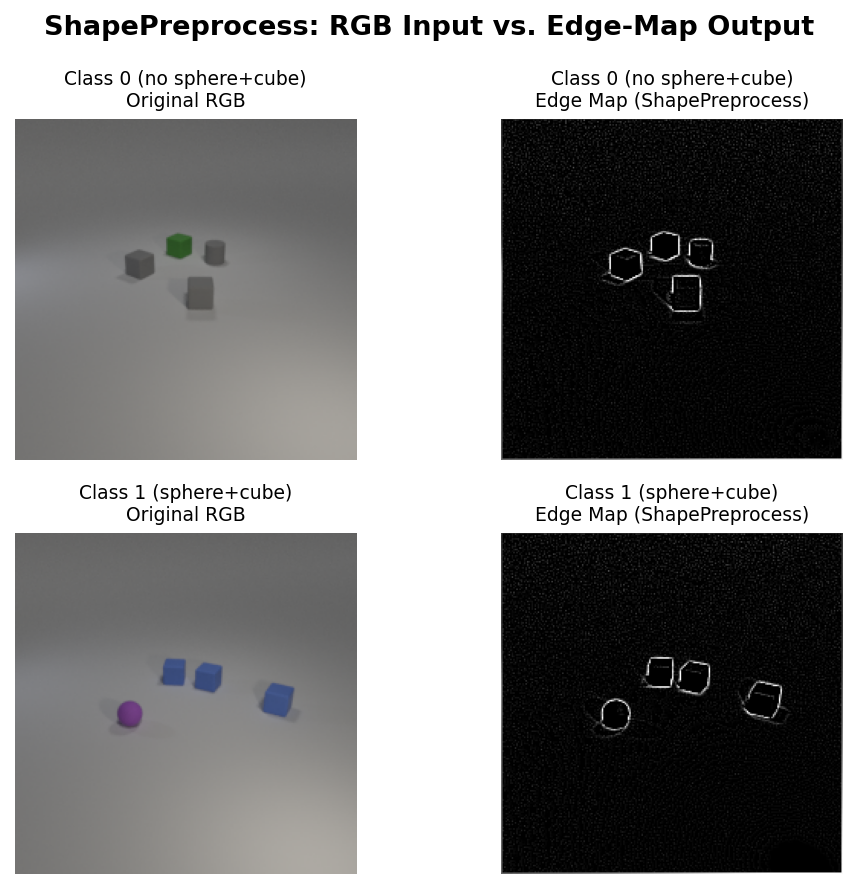
\includegraphics[width=\textwidth,height=0.62\textheight,keepaspectratio]{figures/shapepreprocess_demo.png}\\
      \smallskip
      {\scriptsize \textit{Left}: original RGB.\quad \textit{Right}: edge map.
       Class\,1 (bottom) shows circular sphere outline + rectangular cube corners.}
    \end{column}
  \end{columns}
\end{frame}

% ═══════════════════════════════════════════════════════════════════════
\section{Architecture}
% ═══════════════════════════════════════════════════════════════════════

\begin{frame}[t]{Architecture Overview}
  \centering
  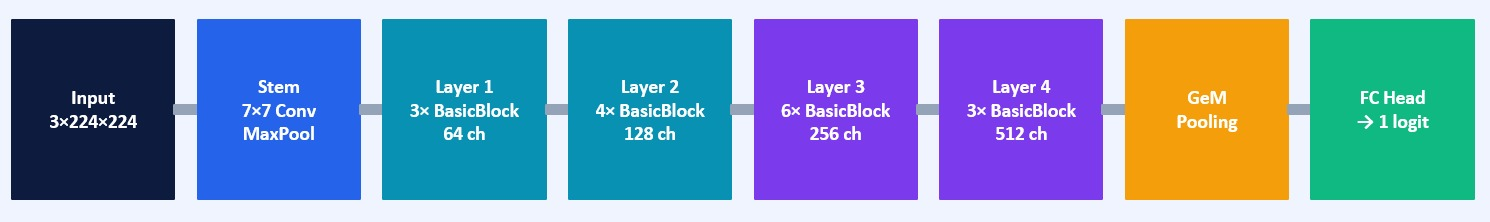
\includegraphics[width=0.92\textwidth,height=0.72\textheight,keepaspectratio]{figures/architecture-block-diagram.jpeg}\\
  \smallskip
  {\small
  \textbf{Stem} (Conv7$\times$7–BN–ReLU–MaxPool)
  $\to$ \textbf{4 Stages} (3-4-6-3 blocks, 64/128/256/512 ch)
  $\to$ \textbf{GeM Pool} $\to$ \textbf{FC Head} $\to$ 1 logit
  }
\end{frame}

\begin{frame}[t,shrink=12]{Architecture Details}
  \begin{columns}[T]
    \begin{column}{0.48\textwidth}
      \begin{block}{BasicBlock (ResNet-34 schedule)}
        \footnotesize
        \begin{enumerate}
          \item Conv1: $3{\times}3$ Conv–BN–\textbf{ReLU}
          \item Conv2: $3{\times}3$ Conv–BN (no ReLU)
          \item \textbf{CBAM} attention
          \item \textbf{DropPath} (stochastic depth)
          \item Add shortcut $\to$ \textbf{ReLU}
        \end{enumerate}
      \end{block}
      \smallskip
      \begin{block}{CBAM}
        \footnotesize
        \textbf{Channel:}\;
        $\mathbf{w}_c = \sigma\!\bigl(\mathrm{MLP}(\bar{\mathbf{x}}_{\mathrm{avg}})
          + \mathrm{MLP}(\bar{\mathbf{x}}_{\mathrm{max}})\bigr)$\\[3pt]
        \textbf{Spatial:}\;
        $\mathbf{w}_s = \sigma\!\bigl(\mathrm{Conv}_{7\times7}(
          [\mathbf{x}_{\mathrm{avg}};\mathbf{x}_{\mathrm{max}}])\bigr)$
      \end{block}
    \end{column}
    \begin{column}{0.48\textwidth}
      \begin{block}{GeM Pooling (learnable $p$, init 3)}
        \footnotesize
        $\mathbf{f} = \bigl(\tfrac{1}{HW}\sum_{h,w} x_{h,w}^{p}\bigr)^{1/p}$\\[2pt]
        Emphasises most-activated positions.\\
        Outperforms ConcatPool2d on this dataset.
      \end{block}
      \smallskip
      \begin{block}{Stochastic Depth (DropPath)}
        \footnotesize
        $p_l = \tfrac{l-1}{L-1}\cdot p_{\max},\quad l=1,\ldots,16,\quad p_{\max}=0.1$\\[2pt]
        First block never dropped; linearly scales to $p_{16}=0.1$.
      \end{block}
      \smallskip
      \begin{block}{Classifier Head}
        \footnotesize
        Drop(0.2) $\to$ Linear(512,256) $\to$ ReLU $\to$ Drop(0.1) $\to$ Linear(256,1)
      \end{block}
    \end{column}
  \end{columns}
\end{frame}

% ═══════════════════════════════════════════════════════════════════════
\section{Training Strategy}
% ═══════════════════════════════════════════════════════════════════════

\begin{frame}[t,shrink=18]{Training Strategy}
  \begin{columns}[T]
    \begin{column}{0.50\textwidth}
      \begin{block}{Two-Phase Training}
        \footnotesize
        \textbf{Phase 1 — Validation training}
        \begin{itemize}
          \item Train on 85\% split, early stopping (patience 20)
          \item Grid-search threshold on 15\% held-out set (401 steps, $[0.05, 0.95]$)
        \end{itemize}
        \textbf{Phase 2 — Full retrain}
        \begin{itemize}
          \item Same seed, 100 epochs on all 18k images
          \item Apply Phase-1 threshold to test predictions
        \end{itemize}
      \end{block}
      \smallskip
      \begin{block}{Optimiser \& Schedule}
        \footnotesize AdamW, $\eta_0\!=\!7{\times}10^{-4}$, $\lambda\!=\!10^{-4}$\\
        5 warm-up epochs + cosine annealing; grad clip 1.0; AMP
      \end{block}
      \smallskip
      \begin{block}{TTA}
        \footnotesize Original + horizontal flip $\to$ average sigmoid outputs\\
        Consistent $\approx\!0.5\%$ gain at near-zero cost
      \end{block}
    \end{column}
    \begin{column}{0.47\textwidth}
      \begin{block}{Key hyperparameters}
        \footnotesize
        \begin{tabular}{ll}
          \toprule
          Parameter & Value \\
          \midrule
          Image size      & $224\times224$ \\
          Batch size      & 128 \\
          Max epochs      & 100 \\
          Learning rate   & $7\times10^{-4}$ \\
          Drop path rate  & $0\to0.1$ (linear) \\
          Dropout         & 0.2 / 0.1 \\
          Random seed     & 42 (single) \\
          \bottomrule
        \end{tabular}
      \end{block}
    \end{column}
  \end{columns}
\end{frame}

% ═══════════════════════════════════════════════════════════════════════
\section{Results}
% ═══════════════════════════════════════════════════════════════════════

\begin{frame}[t,shrink=5]{Training Dynamics \& Threshold Calibration}
  \begin{columns}[T]
    \begin{column}{0.55\textwidth}
      \centering
      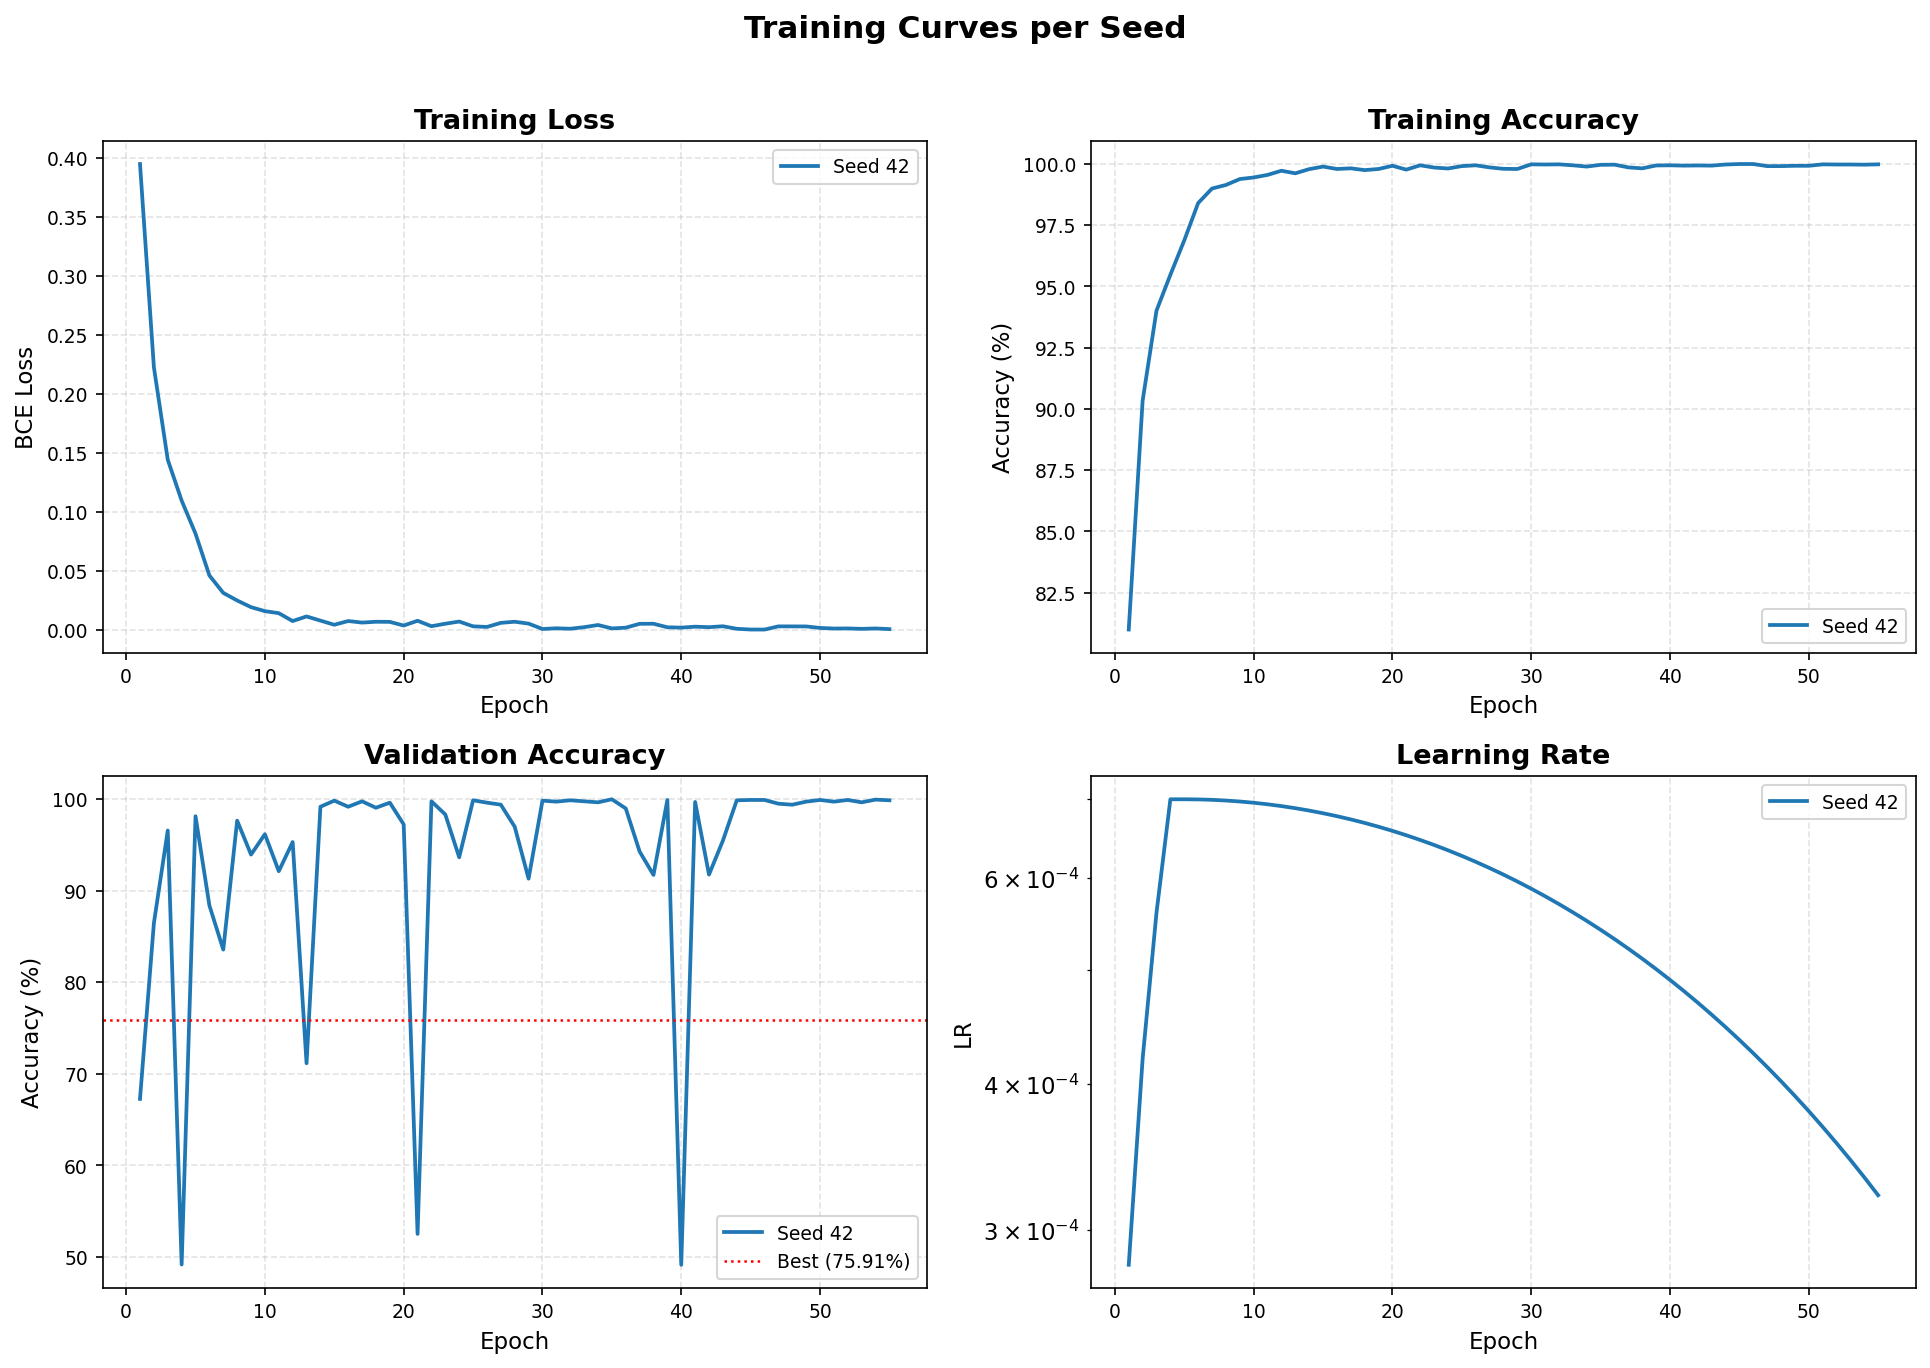
\includegraphics[width=\textwidth,height=0.68\textheight,keepaspectratio]{figures/training_curves.png}\\
      {\footnotesize Steady convergence; val tracks train after warm-up.
       Red dotted line = prior single-model best (75.91\%).}
    \end{column}
    \begin{column}{0.43\textwidth}
      \centering
      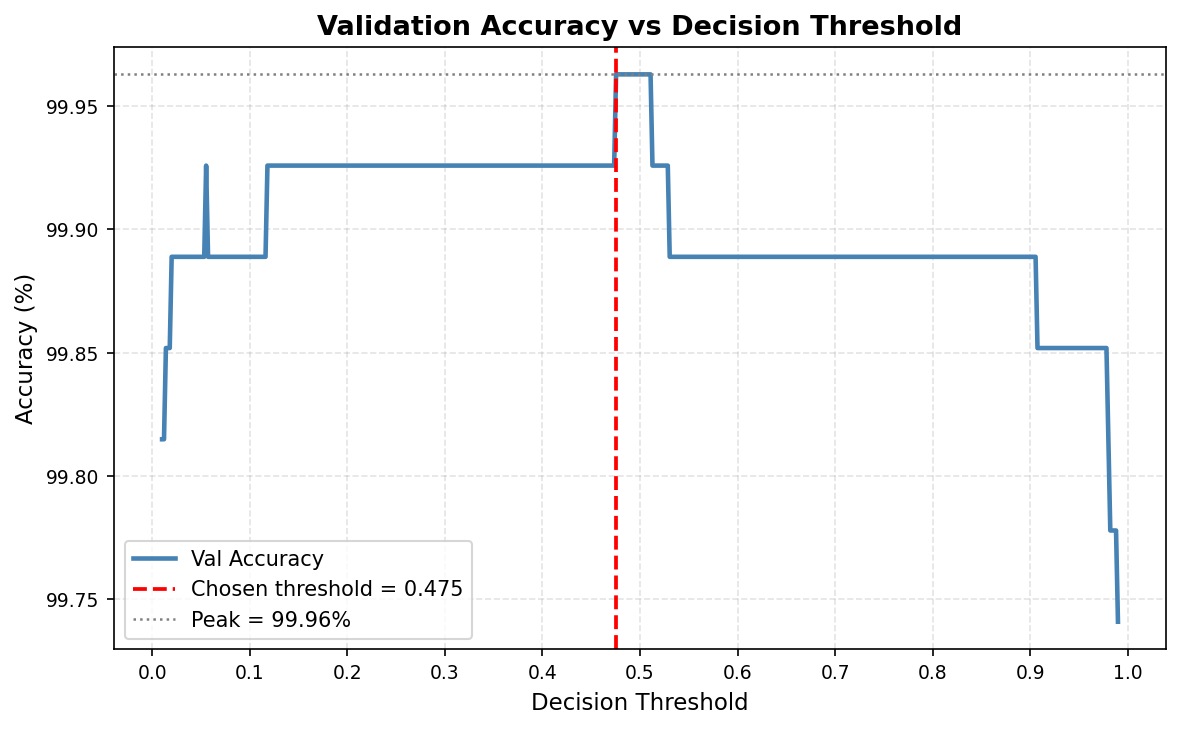
\includegraphics[width=\textwidth,height=0.68\textheight,keepaspectratio]{figures/threshold_sensitivity.png}\\
      {\footnotesize Optimal threshold $\ll 0.5$; post-hoc calibration is essential for edge-map inputs.}
    \end{column}
  \end{columns}
\end{frame}

\begin{frame}[t,shrink=5]{Evaluation Metrics}
  \begin{columns}[T]
    \begin{column}{0.50\textwidth}
      \centering
      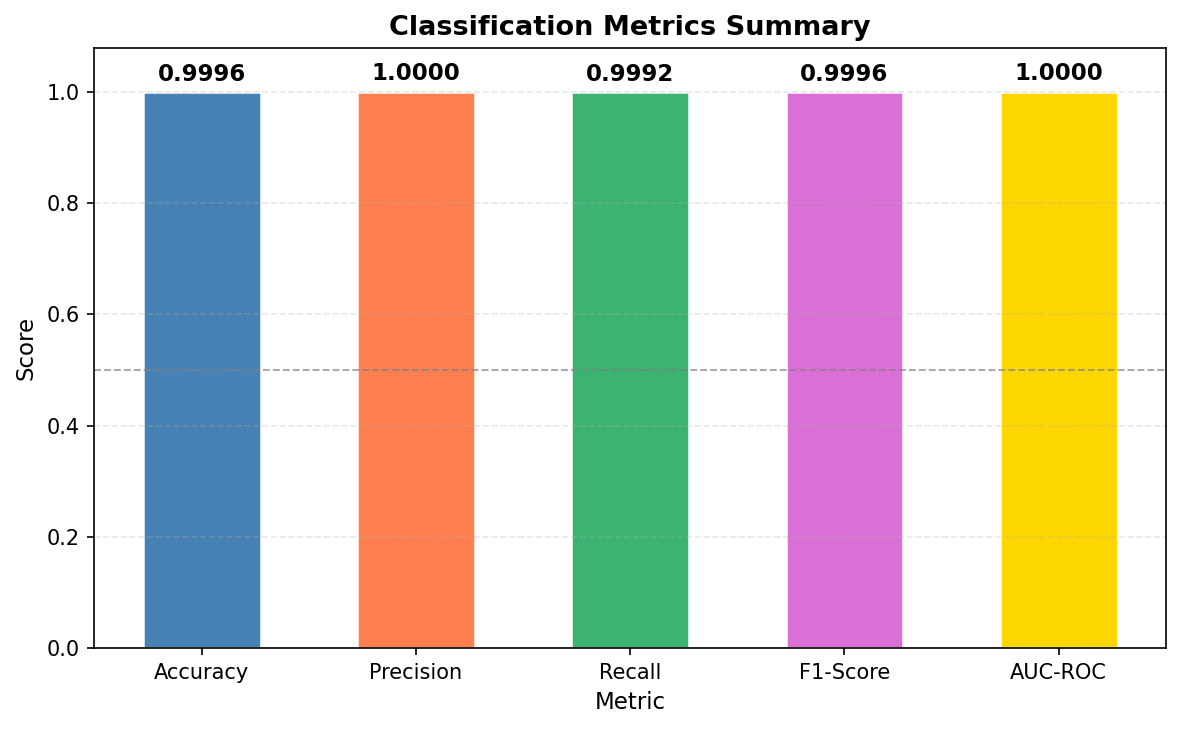
\includegraphics[width=\textwidth,height=0.38\textheight,keepaspectratio]{figures/classification_metrics.png}\\
      \smallskip
      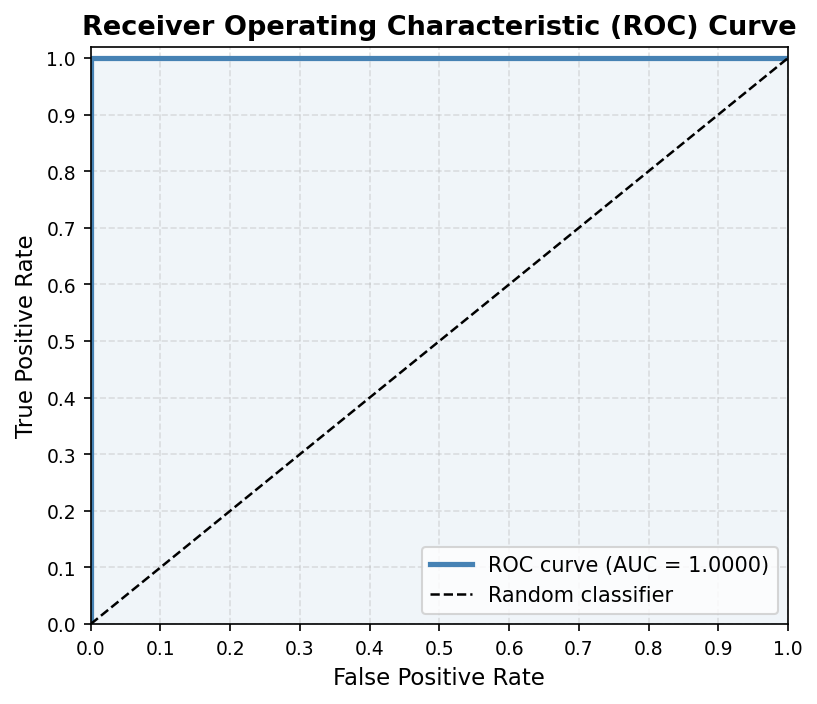
\includegraphics[width=0.48\textwidth,height=0.28\textheight,keepaspectratio]{figures/roc_curve.png}\hfill
      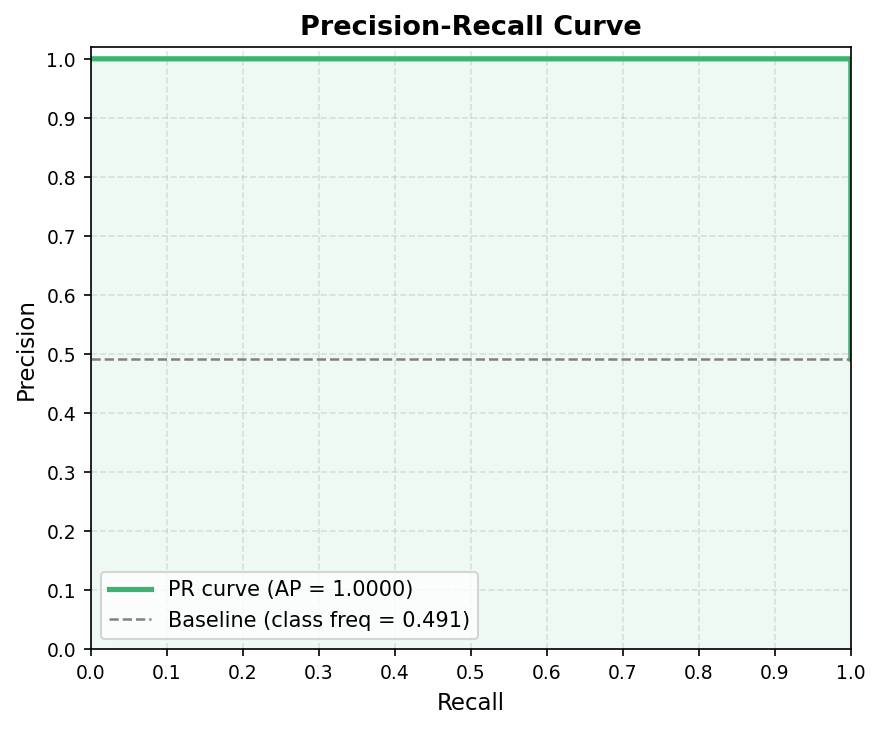
\includegraphics[width=0.48\textwidth,height=0.28\textheight,keepaspectratio]{figures/precision_recall_curve.png}
    \end{column}
    \begin{column}{0.48\textwidth}
      \centering
      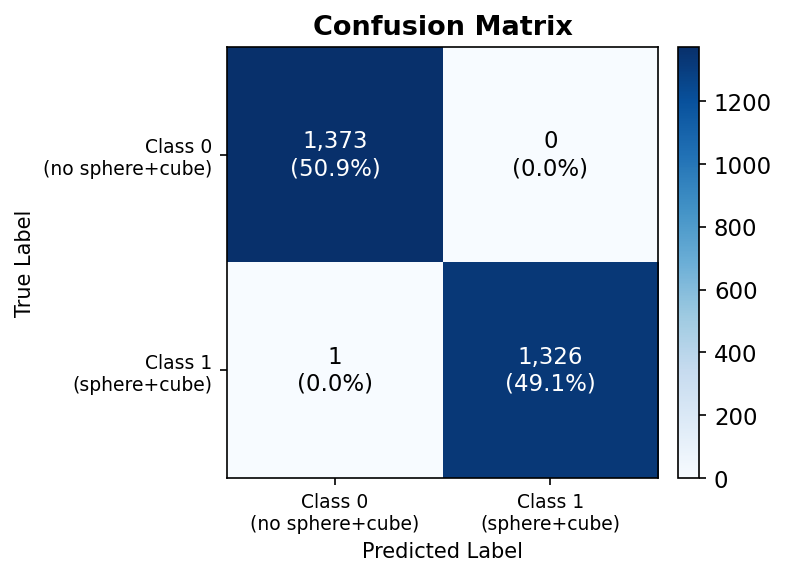
\includegraphics[width=0.85\textwidth,height=0.48\textheight,keepaspectratio]{figures/confusion_matrix.png}\\
      \smallskip
      \begin{block}{\centering Public Leaderboard Score}
        \centering
        \Large\textbf{\alert{0.775311}}\normalsize\ (77.53\%)\\[2pt]
        \footnotesize 5,010 test predictions $\cdot$ seed 42
      \end{block}
    \end{column}
  \end{columns}
\end{frame}

% ═══════════════════════════════════════════════════════════════════════
\section{Ablation}
% ═══════════════════════════════════════════════════════════════════════

\begin{frame}[t,shrink=8]{Score Progression}
  \begin{center}
    \small
    \begin{tabular}{lcc}
      \toprule
      Key Change & Description & LB Score \\
      \midrule
      Baseline                   & Initial submission           & 0.750872 \\
      GeM + Stochastic Depth     & Better pooling + reg.        & 0.759102 \\
      Heavy Reg (MixUp, CutMix)  & Over-regularised             & 0.752867 \\
      Rollback + TTA             & Light aug, hflip TTA         & 0.755860 \\
      100 epochs, 3-seed ensemble & Budget + ensemble           & 0.768827 \\
      \midrule
      \textbf{ShapePreprocess}   & \textbf{Edge-map, single seed} & \alert{\textbf{0.775311}} \\
      \bottomrule
    \end{tabular}
  \end{center}
  \smallskip
  \begin{block}{Key insight}
    \small Prior best 0.768827 used a \textbf{3-seed ensemble}.
    Final 0.775311 beats it with a \textbf{single seed} via ShapePreprocess:
    \alert{better input representation $>$ ensemble diversity}.
  \end{block}
\end{frame}

\begin{frame}[t]{Key Observations}
  \begin{columns}[T]
    \begin{column}{0.48\textwidth}
      \begin{alertblock}{What hurts}
        \footnotesize
        \begin{itemize}
          \item \textbf{RandomResizedCrop}: silently corrupts labels by excluding objects
          \item \textbf{MixUp / CutMix}: destroy the sharp edge signal
          \item \textbf{Label smoothing}: penalises confidence on an unambiguous task
          \item \textbf{EMA}: catastrophic failure (0.495 score)
          \item \textbf{3-seed ensemble} on same split: averaging adds noise on correlated models
        \end{itemize}
      \end{alertblock}
    \end{column}
    \begin{column}{0.48\textwidth}
      \begin{block}{What works}
        \footnotesize
        \begin{itemize}
          \item \textbf{ShapePreprocess}: eliminates colour bias, directly exposes shape signal
          \item \textbf{GeM pooling}: better than average or concat pooling
          \item \textbf{TTA} (hflip): consistent $\approx\!0.5\%$ gain
          \item \textbf{Threshold calibration}: optimal threshold well below 0.5 on edge-map inputs
          \item \textbf{Light regularisation}: dropout 0.2, drop\_path 0.1
        \end{itemize}
      \end{block}
    \end{column}
  \end{columns}
\end{frame}

% ═══════════════════════════════════════════════════════════════════════
\section{Conclusion}
% ═══════════════════════════════════════════════════════════════════════

\begin{frame}[t,shrink=15]{Conclusion}
  \begin{block}{Summary}
    \footnotesize
    \begin{itemize}
      \item Custom \textbf{ResNet-34-like} CNN (3-4-6-3 blocks) + CBAM + GeM Pooling, trained \textbf{from scratch}
      \item \textbf{ShapePreprocess}: highest-impact change — converts RGB to grayscale edge map, directly encoding the sphere/cube discrimination signal
      \item \textbf{Two-phase training}: threshold calibrated on held-out data; final model trained on all 18k images
      \item \textbf{Public score: \alert{0.775311} (77.53\%)} — +2.4\% over initial baseline, +0.9\% over prior 3-seed ensemble
    \end{itemize}
  \end{block}
  \smallskip
  \begin{columns}[T]
    \begin{column}{0.50\textwidth}
      \begin{block}{Member Contributions}
        \footnotesize
        \textbf{Lochan}: architecture (CBAM, GeM, DropPath), training pipeline, ShapePreprocess, tuning, report\\[3pt]
        \textbf{Harsha}: dataset analysis, classification rule discovery, augmentation experiments, validation, report
      \end{block}
    \end{column}
    \begin{column}{0.46\textwidth}
      \begin{block}{Acknowledgements}
        \footnotesize Prof.\ Srijith P.K., Prof.\ Konda Reddy Mopuri,\\
        and the TAs — CS5480, IIT Hyderabad, 2026
      \end{block}
      \smallskip
      \begin{block}{Reproducibility}
        \footnotesize \texttt{submission.py}, \texttt{seed=42}\\
        5,010 predictions, score $\approx$ 0.7753
      \end{block}
    \end{column}
  \end{columns}
\end{frame}

\end{document}
